\begin{frame}{Background -- Elementary Functions}
    \pause \vspace{-2em}
    \begin{minipage}[t]{0.48\linewidth}
        \begin{definition}[%Elementary functions,
                           \citep{OrdinaryDifferentialEquations_Morris_Tenenbaum_1985}]
            The \textbf{elementary functions} on $\Reals$  are partial functions defined by expressions built up from 
            \pause

            \kern-1ex
            \begin{itemize}
                \setlength\itemsep{-1pt}
                \item computable reals, and
                \item the variable $x$,
            \end{itemize}
            \kern-1ex
            \pause by applying (repeatedly) the basic operations below on elementary functions $f,g$:
            \pause
            \begin{itemize}
                \setlength\itemsep{-1pt}
                \item $(f+g)(x) = f(x) + g(x)$ 
                \item $(f\cdot g)(x) = f(x)g(x)$
                \item $\mathrm{inv}_f(x) = \frac{1}{f(x)}$ \kern5em where $\frac{1}{0} =\ \uparrow$
                \item $\mathrm{root}_{n,f}(x) = \sqrt[n]{f(x)}$ \hfill where $0< n \in \Nats$
                \item $\ln_f(x) = \ln(f(x))$
                \item $\exp_f(x) = e^{f(x)}$
                \item $\sin_f(x) = \sin(f(x))$
                \item $\arcsin_f(x) = \arcsin(f(x))$
            \end{itemize}
        \end{definition}
    \end{minipage}
    \hfill
    \pause \begin{minipage}[t]{0.45\linewidth}
        \begin{exampleblock}{\textbf{\textcolor{BrickRed}{Problem}}}
            The domains of elementary functions are not all open!
        \end{exampleblock}
        \pause
        \begin{exampleblock}{\color{OliveGreen}\textbf{Solution: Modifications}}
            \pause
            \begin{itemize}
                \item We define $\sqrt[n]{x} = 0$ for $x < 0$ when $n$ is even.
                \pause \item We extend the definition of $\arcsin(x)$ to be $\frac{\pi}{2}$ for $x > 1$ and to be $-\frac{\pi}{2}$ for $x<-1$.
            \end{itemize}
        \end{exampleblock}
        \centering
        \visible<7->{
        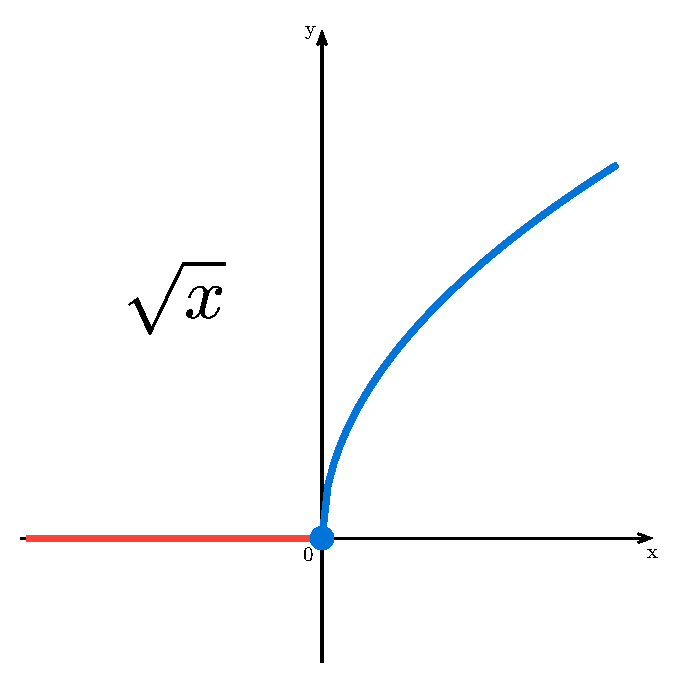
\includegraphics[width=0.35\linewidth]{sqrt.pdf}
        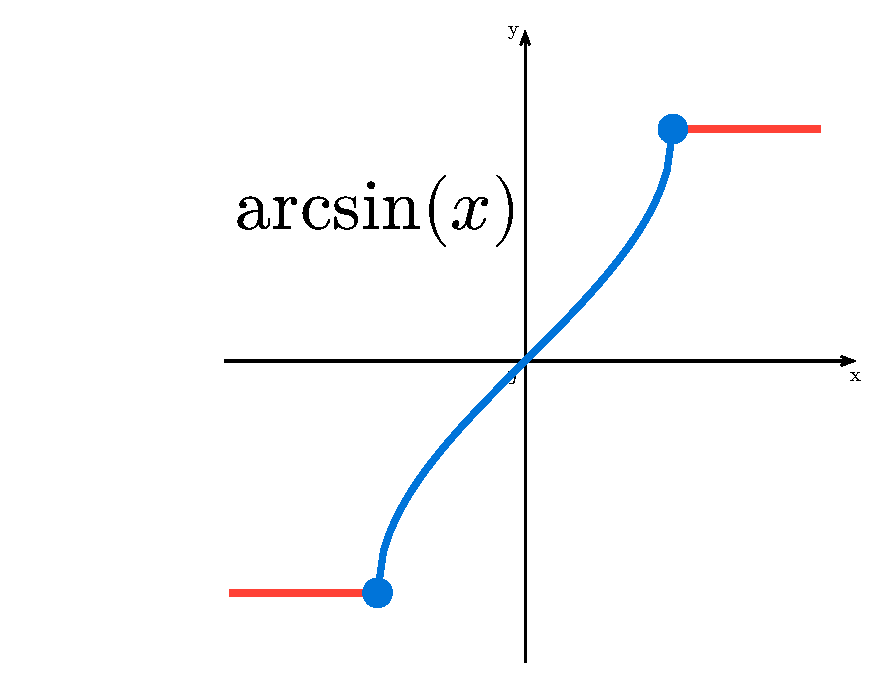
\includegraphics[width=0.35\linewidth]{arcsin.pdf}}
    \end{minipage}\kern-0.2em
\end{frame}